\documentclass[a4paper]{article}
\usepackage{preamble}

% Setup title
\title{PHYSICS 2 - TERM 2}
\author{Marc Sanchis}
\date{April 2024 - June 2024}

\begin{document}

% Title
\newgeometry{top=2cm, bottom=5.5cm}
\maketitle

% Table of Contents
\renewcommand{\contentsname}{}
\tableofcontents

% Body
\newpage
\restoregeometry
\pagestyle{fancy}
\setcounter{section}{4}

\newcounter{ex}[section]
\newcounter{prob}[section]
\setcounter{ex}{0}
\setcounter{prob}{0}

\section{Magnetism in Matter}

\subsection{Magnetic Behaviour}
Materials fall into three groups based on their magnetic behaviour:

\begin{itemize}
    \item \textbf{Diamagnetic}: It has a weak, opposite-direction reaction to a $B$ field.
    \item \textbf{Paramagnetic}: With no $B$ their electrons have a defined magnetic moment, and when a magnetic field is applied, they have a slight attraction towards it.
    \item \textbf{Ferromagnetic}: Same as Paramagnetic, but its dipoles are aligned even before the $B$ the field is applied and has a very strong, attractive reaction.
\end{itemize}

For $B_{0}=0$, the vacuum has $(\vec{m}=\vec{0}, \vec{B}=\vec{0})$, Diamagnetic $(\vec{m}_{atomic}=\vec{0}, \vec{m}=\vec{0},\vec{B}=\vec{0})$, Paramagnetic $(\vec{m}_{atomic}\neq \vec{0},\vec{m}=\vec{0}\vec{B}=\vec{0})$, Ferromagnetic $(\vec{m}_{atomic}\neq\vec{0},\vec{m}\neq\vec{0}),\hspace{1ex}\vec{0}\in D:\sum\vec{m}$ .

For $B_{0}\neq 0$, the vacuum has $\vec{B}_{total}=\vec{B}_{0}$, Diamagnetic $\vec{B}_{total}<\vec{B}_{0}$, Paramagnetic $\vec{B}_{total}>\vec{B}_{0}$, Ferromagnetic $\vec{B}_{total}\gg \vec{B}_{0}$ .

\begin{align}
\vec{M}=\frac{d\vec{m}}{dv},\hspace{4ex}J_{S}&=|\vec{M}|,\hspace{4ex}dm=dI\cdot dS \\
\vec{B}_{total}&=\vec{B}_{0}+\vec{B}_{JS}
\end{align}

\note{If the magnetisation $M$ is constant, amperian bound currents appear in the material surface}
\begin{figure}[h]
    \centering
    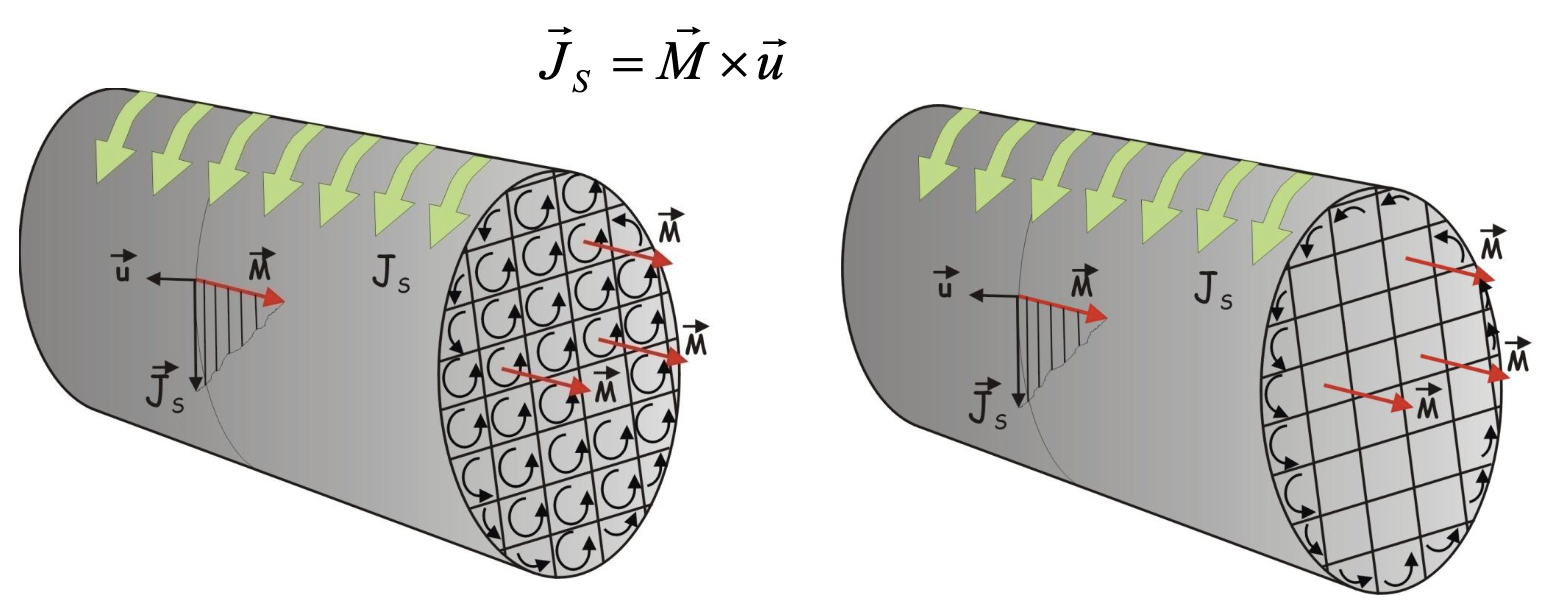
\includegraphics[width=0.5\textwidth]{IMG/js.png}
    \caption{Amperian bound currents appearing}
    \label{fig:js}
\end{figure}

\subsection{Magnetic Excitation}
\subsubsection{The H field}
The $H$ field only depends on the free current.
$$
\vec{H}=\frac{\vec{B}}{\mu_{0}}-\vec{M}, \hspace{4ex}\vec{B}=\mu_{0}(\vec{H}+\vec{M})\to B^*=\mu_{0} (H+M)
$$
$H$ can be demonstrated in two equivalent ways:
$$
\begin{cases}
&\oint \vec{H}\cdot d\vec{l}=\int_{C} \frac{\vec{B}}{\mu_{0}} \, d\vec{l}\,-\int_{C}^{} \vec{M} \, d\vec{l}\, = \frac{1}{\mu_{0}}[\mu_{0}nlI+\mu_{0}J_{S}l]-J_{S}l=nlI \\
&\oint_{C} \vec{H}\cdot d\vec{l}=Hl
\end{cases} \hspace{1ex}\to \boxed{H=nI}
$$
and
$$
\to\begin{cases}
B=\mu_{0}[nI+J_{S}]=\mu_{0}[nI+M] \\
B^*=\mu_{0}(H+M)
\end{cases}\hspace{1ex}\to \boxed{H=nI}
$$

\subsubsection{Ampère's Theorem for H}
Per Ampère's theorem for $H$:
$$
\oint_{C}\vec{H}\cdot d\vec{l}=I_{f r e e}, \hspace{4ex}Curl(\vec{H})=\vec{J}_{f r e e}
$$

\subsubsection{M-H Relationship}
The relationship between $M$ and $H$ is
$$
\vec{M}=\chi \vec{H}
$$
For diamagnetic materials $0<\chi\ll-1$, paramagnetic $0>\chi\ll 1$, ferromagnetic $1000<\chi<8000$.

$$
\vec{H}=\frac{\vec{B}}{\mu_{0}}-\vec{M}=\frac{\vec{B}}{\mu_{0}}-\chi \vec{H} \to \vec{B}=\mu_{0}(1+\chi)\vec{H}=\mu \vec{H}
$$
$$
\mu_{r}=\frac{\mu}{\mu_{0}}=1+\chi
$$

\stepcounter{prob}\vspace{2ex}\textbf{\textit{Prob.\thesection.\theprob: }}PB.6 Cylindrical tube of radius $r_{1},\,r_{2}$ and a charged conductive wire through the inside.
$$r_{1}=4mm,\,r_{2}=6mm,\,\chi=3\times 10^{-4},\,A=0,5A$$

$\triangleright$ a) Equivalent currents for the walls
\begin{align}
\oint\vec{H}d\vec{l}=I\implies \vec{M}&=\lambda \vec{H}\implies \vec{J}_{S}=\vec{M}\times \vec{u} \\
\text{Ampère's T. }\to Hl&=I\implies H =\frac{I}{2\pi r} \\
\end{align}
$$
\begin{cases}
M=0, & r<a,\,r>b \\
M=\chi \frac{I}{2\pi r}, & a<r<b\implies\vec{J}_{s}=\vec{M}\times \vec{u}\begin{cases}
r=r_{1}&\implies J_{Sr_{1}}=\chi \frac{I}{2\pi r_{1}} \\
r=r_{2}&\implies J_{Sr_{2}}=\chi \frac{I}{2\pi r_{2}}
\end{cases}
\end{cases}
$$
\begin{align}
J_{Sr_{1}}=3\times 10^{-4} \frac{0'5}{2\pi\, 4\times 10^{-3}}=\boxed{5'96\times 10^{-3}A / m} \\
J_{Sr_{2}} = 3\times 10^{-4} \frac{0'5}{2\pi\,6\times 10^{-3}}=\boxed{3'98 \times 10^{-3} A / m}
\end{align}
$\triangleright$ b) $B(r)$ for $b<r<c,\,r>c$
\begin{align}
\vec{B}=\mu \vec{H}=\mu _{r}\mu_{o}\vec{H} & =\mu_{o}(\chi+1)\vec{H}
\end{align}
$$
\begin{cases}
b<r<c,&B_{1}=\mu_{o}(\chi H) \frac{I}{2\pi r} \\
r>c,&B_{2}=\mu_{o}H
\end{cases}
$$
\begin{align}
B_{1}&=4\pi \times 10^{-7}(3\times 10^{-4}+1) \frac{0'5}{2\pi r}=\boxed{\frac{10^{-7}}{r}\,T} \\
B_{2}&=4\pi \times 10^{-7} \frac{0'5}{2\pi r}=\boxed{\frac{10^{-7}}{r}\,T}
\end{align}
\subsection{Ferromagnetism}
\setcounter{equation}{0}
A ferromagnetic material has the property $\mu\gg$ and by \textit{Ampère's Theorem} on a coiled toroid
$$
\oint_{C}\vec{H}d\vec{l}=I\implies H_{2}\pi r=NI\implies \boxed{H=\frac{NI}{2\pi r}}
$$
so we can see $H$ is linear with $I$, but $H$ is not linear with $B$ and $M$, because $\mu \neq \text{const}$, the curve describing this relation is the \textit{First Magnetisation Curve}.
$$
H\propto I,\hspace{4ex}\mu=B / H\implies 
$$

\begin{figure}[H]
    \centering
    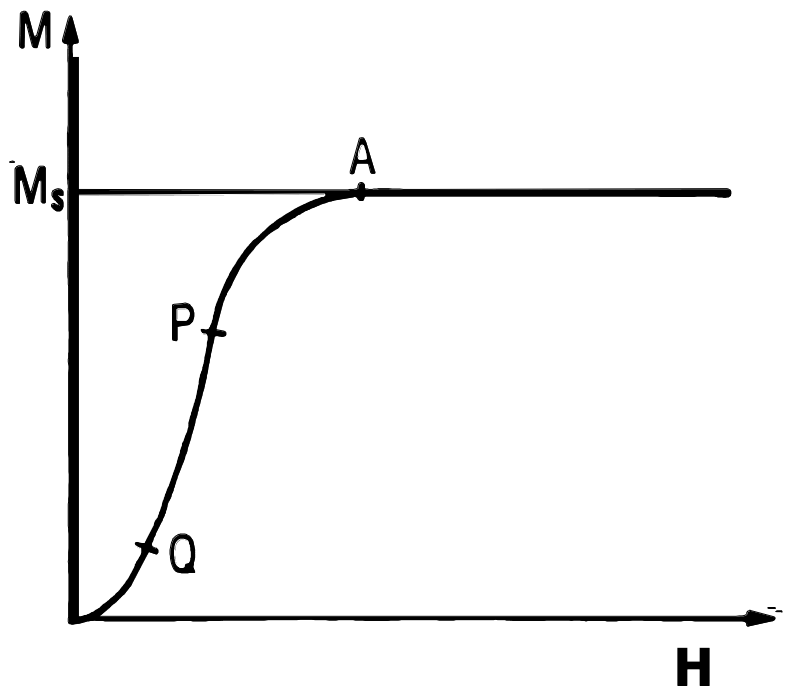
\includegraphics[width=0.33\textwidth]{IMG/mag_curve.png}
    \caption{Magnetisation curve}
    \label{fig:mag_curve}
\end{figure}

For any case different from the first excitation will not go through $M\cap H=0$, this is called the \textit{Hysteresis Cycle}.

\begin{figure}[H]
    \centering
    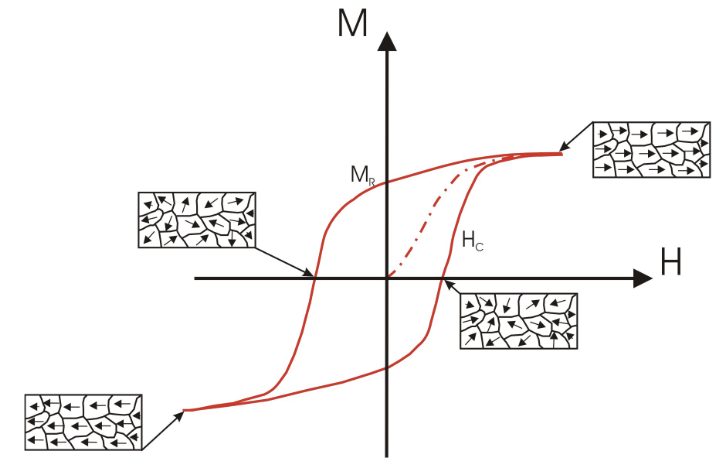
\includegraphics[width=0.33\textwidth]{IMG/hyst_cycle.png}
    \caption{Hysteresis cycle}
    \label{fig:hyst_cycle}
\end{figure}

A ferromagnetic material can be returned to its initial state by using constantly smaller secondary hysteresis cycles.

\subsection{Permanent Magnets}
\setcounter{equation}{0}
A magnetic cylinder can be calculated like a solenoid and vice versa, as $n=J_{S}=M$
\begin{align*}
&\text{Solenoid }\to & B&=\frac{\mu_{o}nI}{2}(\sin \phi_{2}-\sin \phi_{1}) \\
& \text{Cylinder }\to & B&=\frac{\mu _{o}J_{S}}{2}(\sin \phi_{2}-\sin \phi_{1})=\frac{\mu_{o}M}{2}(\sin \phi_{2}-\sin \phi_{1})
\end{align*}
this way $H$ can be obtained on the inside
\begin{align*}
H_{\text{in}}&=\frac{\mu_{o}M}{2\mu_{o}}(\sin \phi_{2}-\sin \phi_{1})-M= \\
&=\frac{H}{2}((\sin \phi_{2}-\sin \phi_{1})-2)<0
\end{align*}
so $H$ runs in the opposite way inside the magnet to let $M$ manifest, nevertheless, on the outside $\vec{H}\parallel \vec{B}$ 
$$
H_{\text{out}}=\frac{M}{2}(\sin \phi_{2}-\sin \phi_{1})
$$
\stepcounter{ex}\vspace{2ex}\textbf{\textit{Ex.\thesection.\theex: }}PB.8 A permanent magnet with a ring form with a gap $e=2mm$ and a medium radius $r=10cm$, the magnetic field in the gap is $B=0'02T$.

$\triangleright$ a) Magnetic excitation inside the magnet
\begin{align}
\text{Ampère's T. }\to \oint_{C}\vec{H}d\vec{l}=I_{\text{inter}} =0
\end{align}
\vspace{1ex}\note{$H$ is not null, as the magnet has magnetisation of its own, while the currents are non-existent}\vspace{1ex}

\begin{align}
H_{\text{Fe}}&=H_{e} \frac{e}{l_{\text{Fe}}}=\frac{B_{e}}{\mu_{o}} \frac{e}{2\pi r-e} \\
&=-15915'49\cdot \frac{2\times 10^{-3}}{(2\pi \cdot 10\times 10^{-2}-2\times 10^{-3})} \\
&=\boxed{-50'8 A / m}
\end{align}

$\triangleright$ b) Magnetisation of the magnet

The field in the gap is the same as the field of the magnet; the flux can prove this
\begin{align}
\phi=\int \vec{B}d\vec{S}\, =B_{\text{Fe}}S_{\text{Fe}}=B_{e}F_{e}\implies B_{\text{Fe}}=B_{e}
\end{align}

For the magnetisation, we can use the excitation formula
\begin{align}
\vec{H}_{\text{Fe}}&=\frac{\vec{B}_{e}}{\mu_{o}}-\vec{M} =\frac{0'02}{4\pi \times 10^{-7}}-\vec{M}=-50'8 \\
M&=\frac{0'02}{4\pi \times 10^{-7}} -H=\boxed{1'6\times 10^{4}A / m}
\end{align}
\subsubsection{Ampère's Theorem With the Flux Prove of Gap-Magnet Magnetic Equality}
\setcounter{equation}{0}
If we divide the gapped magnet into four sections, we get
\begin{align}
\oint_{C}\vec{H}d\vec{l}=I\implies H_{1}l_{1}+H_{2}l_{2}+H_{3}l_{3}+H_{4}l_{4}+H_{e}l_{e}
\end{align}
therefore either $I$ or $B$ and $\mu_{1},\,\mu_{2},\,\mu_{3},\,\mu_{4}$ must be known. If only $B_{e}$ and the $\mu$ of the sections, we can prove the \textit{gap-magnet magnetic field equality}
\begin{align}
\phi=\int _{S}\vec{B} \, d\vec{S}\, &\implies B_{1}S=B_{2}S=B_{3}S=B_{4}S=B_{e}S \\
&\implies B_{1}=B_{2}=B_{3}=B_{4}=B_{e} 
\end{align}
\subsection{Magnetic Circuits}
\setcounter{equation}{0}
A magnetic circuit includes a ferromagnetic material with a magnetic field induced by a current; it transforms electricity in magnetisation.

\begin{figure}[H]
    \centering
    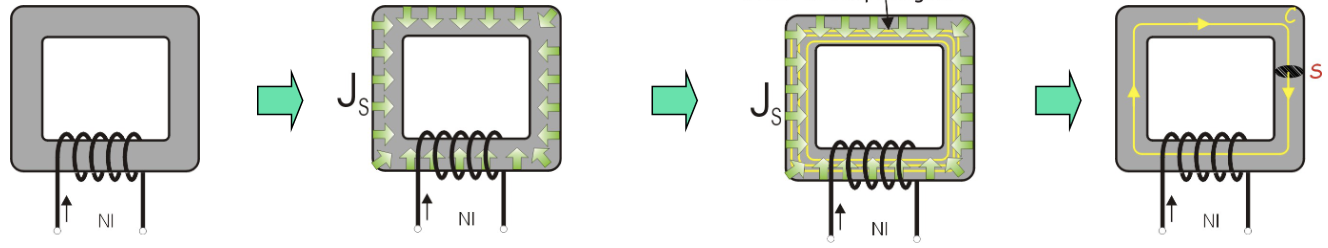
\includegraphics[width=\textwidth]{IMG/mag_circuit.png}
    \caption{Caption}
    \label{fig:enter-label}
\end{figure}

\subsubsection{Hopkinson's Law}
\setcounter{equation}{0}
By adapting \textit{Ampère's Theorem}, we get a new law that rules magnetic circuits
$$
\oint_{C}\vec{H}d\vec{l}=\oint_{C}Hdl=\oint_{C}\frac{B}{\mu}dl=\oint \frac{\phi}{\mu S}dl=\phi \oint \frac{dl}{\mu S}=\phi \cdot R=NI
$$
$$
\text{Hopkinson's Law}\to \boxed{\phi \cdot R=NI=F}
$$


\end{document}
